\documentclass[parskip=full]{scrartcl}
\usepackage[T1]{fontenc}    % avoid garbled Unicode text in pdf
\usepackage[utf8]{inputenc} % use utf8 file encoding for TeX sources
\usepackage[german]{babel}  % german hyphenation, quotes, etc
\usepackage{hyperref}       % detailed hyperlink/pdf configuration
\hypersetup{                % ‘texdoc hyperref‘ for options
pdftitle={PSE: Entwicklung eines relationalen Debuggers - Pflichtenheft},%
,%
}
\usepackage{graphicx}       % provides commands for including figures
\usepackage{csquotes}       % provides \enquote{} macro for "quotes"
\usepackage[nonumberlist]{glossaries}     % provides glossary commands
\usepackage{enumitem}
\usepackage{xcolor}
\newcommand\frage[1]{\textcolor{red}{#1}}
\renewcommand{\glstextformat}[1]{\textbf{\color{blue}\em #1}}

\newglossaryentry{Debugger}
{
	name={Debugger},
	description={Ein Debugger ist ein Werkzeug zum Diagnostizieren und Auffinden von Fehlern in Computerprogrammen}
}
\newglossaryentry{Variableninspektor}
{
	name={Variableninspektor},
	plural={Variableninspektors},
	description={Zeigt die Variablen des Programms und deren Belegung an}
}
\newglossaryentry{Relationale Eigenschaft}
{
	name={Relationale Eigenschaft},
	plural={Relationale Eigenschaften},
	user1={Relationalen Eigenschaften},
	user3={Relationaler Eigenschaften},
	description={Relationale Eigenschaften sind solche Eigenschaften, die sich auf mindestens zwei Programmausführungen beziehen. Dabei können diese sich auf Variablen aus den verschiedenen Programmläufen beziehen und diese miteinander in Verbindung setzen, etwa ob eine Variable größer als eine andere ist}
}
\newglossaryentry{Interpreter}
{
	name={Interpreter},
	description={Teil des Produkts, welches die definierte Sprache ausführt}
}
\newglossaryentry{Tooltip}
{
	name={Tooltip},
	plural={Tooltips},
	description={Zeigt eine Beschreibung zu einem Element der Benutzeroberfläche}
}

\newglossaryentry{Einzelschritt}
{
	name={Einzelschritt},
	plural={Einzelschritte},
	description={Ein Einzelschritt entspricht einem ausgeführten Befehl in einem Programm.}
}
\newglossaryentry{Schritt}
{
  name={Schritt},
  plural={Schritte},
  description={Der Benutzer kann durch die Schrittgröße festlegen, aus wie vielen Einzelschritten ein Schritt befehlen soll. Die Schrittgröße entspricht also der Anzahl ausgeführter Befehle bei einem Schritt.}
}
\newglossaryentry{Schrittgroesse}
{
	name={Schrittgröße},
	description={Die vom Benutzer anzugebende Schrittgröße bestimmt die pro Schritt ausgeführten Befehle. Hierbei zählt jeder Befehl einzeln und in Methoden und Funktionen werden alle Befehle gezählt, statt die Methode bzw. Funktion als einen Befehl zu betrachten}
}
\newglossaryentry{Step-Out}
{
	name={Step-Out},
	description={Springt bis zum Ende der aktuell ausgeführten Funktion. Befindet sich der Debugger in der main-Funktion, wird das Programm fertig gedebuggt}
}
\newglossaryentry{Step-Over}
{
	name={Step-Over},
	description={Ist der Befehl in der aktuellen Zeile ein Methodenaufruf, wird das Programm bis zum Ende dieser Methode gedebuggt. Ist der Befehl eine einzelne Ausführung,
	wird diese wie bei einem Einzelschritt ausgeführt}
}
\newglossaryentry{Breakpoint}
{
	name={Breakpoint},
	plural={Breakpoints},
	description={Erreicht das Produkt einen Breakpoint, stoppt es an dieser Stelle das Debuggen}
}
\newglossaryentry{Debugging-Prozess} {
	name={Debugging-Prozess},
	plural={Debugging-Prozesse},
	description={Die zu debuggenden Programme wurden einmal komplett gedebuggt.}
}
\newglossaryentry{bedingter Breakpoint}
{
	name={bedingter Breakpoint},
	plural={bedingte Breakpoints},
	user1={bedingten Breakpoints},
	user2={Bedingte Breakpoints},
	description={Der Benutzer kann Relationen zwischen Variablen der zu debuggenden Programme angeben. Sobald diese Relation zutrifft, stoppt das Produkt das Debuggen,
	auch wenn aktuell ein Schritt ausgeführt wird, der weiter springen würde. Weiteres dazu ist in Kapitel 12 zu finden}
}
\newglossaryentry{Watch-Expression}
{
	name={Watch-Expression},
	plural={Watch-Expressions},
	description={Der Benutzer kann Ausdrücke, die sich auf Variablen in den zu debuggenden Programmen beziehen, als Watch-Expressions angeben. Er wird dann beim Debuggen dauerhaft über den aktuellen Zustand des ausgewerteten Ausdrucks informiert. Weiteres dazu ist in Kapitel 12 zu finden}
}
\newglossaryentry{Debugmodus}
{
	name={Debugmodus},
	description={Das Produkt befindet sich im Debugmodus, sobald der Benutzer Start auswählt. Im Debugmodus können Eingabevariablen und die zu debuggenden Programme nicht
	mehr geändert werden}
}
\newglossaryentry{Editiermodus}
{
	name={Editiermodus},
	description={Das Produkt befindet sich im Editiermodus, bevor der Benutzer den Debugmodus startet, und nachdem das Debuggen abgeschlossen ist. Im Editiermodus
	können Eingabevariablen und die zu debuggenden Programme geändert werden}
}
\newglossaryentry{Konfigurationsdatei}
{
	name={Konfigurationsdatei},
	plural={Konfigurationsdateien},
	description={Der Benutzer kann Konfigurationsdateien bezüglich eines Durchlaufs des Produkts erstellen. Diese Dateien enthalten die zu debuggenden Programme,
	Breakpoints, Watch-Expressions, Eingabevariablen, \gls{Schrittgroesse}n und die Stelle, an der das Debuggen eventuell unterbrochen wurde}
}



\let\glsplgen\glsuseri
\let\glsplcap\glsuserii
\let\glsplgenER\glsuseriii

\makeglossaries

\font\myfont=cmr12 at 20pt

\title{
	\vspace{2cm}
	\myfont 
	Praxis der Softwareentwicklung:\\ 
	Entwicklung eines relationalen Debuggers\\
}
\subtitle{
	\vspace{1cm}
	\myfont
	Pflichtenheft
}
\author{
	\vspace{1cm} \\
	Benedikt Wagner\\
	\texttt{udpto@student.kit.edu}
	\and \vspace{1cm} \\ Chiara Staudenmaier\\
	\texttt{uzhtd@student.kit.edu}
	\and Etienne Brunner\\
	\texttt{urmlp@student.kit.edu}
	\and Joana Plewnia\\
	\texttt{uhfpm@student.kit.edu} 
	\and Pascal Zwick\\
	\texttt{uyqpk@student.kit.edu}
	\and Ulla Scheler\\
	\texttt{ujuhe@student.kit.edu}
	\vspace{1cm}
	\and Betreuer: Mihai Herda, Michael Kirsten
	\vspace{4cm}
}


\begin{document}
\clearpage
\maketitle
\pagenumbering{gobble}
\newpage

\tableofcontents
\newpage
\pagenumbering{arabic}
%Eventuell Fußnoten generieren
\section{Produktübersicht}
%kurze Übersicht über das Produkt
Das Produkt \enquote{DIbugger} soll dem Nutzer die Möglichkeit bieten, mehr als ein Programm gleichzeitig zu debuggen und interaktiv zu analysieren. \\
Dabei sollen die Konzepte eines herkömmlichen Debuggers, namentlich \glspl{Einzelschritt}, \glspl{Breakpoint} und Anzeige eines \glspl{Variableninspektor}, erhalten bleiben und um zusätzliche Konzepte, die den Umgang mit zwei oder mehr Programmläufen erleichtern, erweitert werden. Zu diesen Konzepten gehören das Betrachten von sogenannten \glspl{Watch-Expression}, bei denen der Nutzer beispielsweise Differenz oder Quotient zweier Variablen aus den verschiedenen Programmen untersuchen kann. Der Fokus liegt hierbei auf der Unterstützung des Findens von \glsplgen{Relationale Eigenschaft} in den vom Nutzer verfassten Programmen.
Die Sprache dieser Programme wird in Kapitel 12 näher definiert.
\vspace{0.7cm}
\begin{figure}[!h]
\centering

\includegraphics[width=0.6\textwidth]{logo_nongi.png}
\caption{Produktlogo}
\end{figure}

\section{Produkteinsatz}
Die Verifikation \glsplgenER{Relationale Eigenschaft} stellt ein wichtiges Forschungsthema der Theoretischen Informatik dar - und ein unentscheidbares Problem. Folglich ist es nicht immer einfach, einen Beweis zu führen. \\
Dieses Produkt ist darum darauf ausgelegt, dem Nutzer durch die Möglichkeit des gleichzeitigen Debuggens der Programme bei der Beweisführung helfen. Obwohl es speziell anhand der Anforderungen der Mitarbeiter des Instituts für theoretische Informatik am Lehrstuhl \enquote{Anwendungsorientierte formale Verifikation - Prof. Dr. Beckert} am Karlsruher Institut für Technologie entwickelt wird, kann das Produkt von jedem genutzt werden, der ein grundlegendes Verständnis eines Debuggers hat. Um alle Funktionalitäten des Produktes auszuschöpfen, ist ein Grundverständnis logischer Ausdrücke hilfreich.\\

%unterstützt das Institut für theoretische Informatik am Karlsruher Institut für Technologie beim Führen von Beweisen zu \glsplgen{Relationale Eigenschaft} von Programmen. Hierbei soll die 
%Verwendet wird das Produkt hierbei von wissenschaftlichen Mitarbeitern am Lehrstuhl \enquote{Anwendungsorientierte formale Verifikation - Prof. Dr. Beckert} am Karlsruher Institut für Technologie und soll in deren Büroumgebung zum Einsatz kommen. 

%Anwendungsbereiche, Zielgruppen, Betriebsbedingungen
 

\section{Produktumgebung}
%Software, Hardware, Orgware, Schnittstellen
Das Produkt läuft auf dem Rechner des Nutzers und benötigt keine Kommunikation zu anderen Rechnern. Hierbei läuft das Produkt eventuell neben anderen Applikationen, kommuniziert jedoch nicht mit diesen.

\subsection{Software}
Da es sich bei dem Produkt um ein Java-Programm handelt, muss ein JRE (Java Runtime Environment) der Version 8 oder höher auf dem Rechner vorhanden sein oder mitinstalliert werden. \\
Das Produkt läuft sowohl auf Windows (Vista SP2, 7, 8.x, 10), als auch auf Mac OS X (10.8.3+, 10.9+) und Linux (15.10 Kernel 4.2 oder höher) (64bit empfohlen).

\subsection{Hardware}
An die Hardware des Rechners werden keine speziellen Anforderungen neben den Anforderungen für Java 8 gestellt. Das Produkt wird auf Rechnern mit folgender Hardware getestet: \\ \\
\begin{tabular}{l||c|c|c}
   	& Betriebssystem & Prozessor & RAM \\
	\hline
	\hline
	Rechner 1 & Windows 7 64bit & AMD Phenom II X4 B50 4K 4T @3.5Ghz & 10GB DDR3 \\
	Rechner 2 & Windows 7 64bit & Intel Core i3-380M 2K 4T @2.5Ghz & 8GB DDR3 \\
	 & KDE Neon 5.11.3 64bit &  \\
	Rechner 3 & Ubuntu 17.04 64bit & Intel Core i5-7200U @3.1Ghz & 8GB DDR3 \\
	Rechner 4 & Windows 10 Pro 64bit & Intel Core i7-7500U @2.7Ghz & 16GB DDR4\\
		& Ubuntu 17.04 64bit\\
\end{tabular}
\newpage
\subsection{Schnittstellen}
Als Schnittstelle zum Nutzer selbst dient die graphische Benutzeroberfläche. \\ Es können sowohl Sprachkonfigurationsdateien, die die auf dieser Oberfläche angezeigten Texte beeinflussen, als auch Einstellungsdateien, die Einstellungen des Nutzers speichern, und Dateien, die Eingaben des Nutzers festhalten, geladen und persistent gespeichert werden. Um dies zu ermöglichen, nutzt das Produkt die in Java 8 vorhandenen Schnittstellen zum Dateisystem des Betriebssystems. 


\section{Produktfuntionen}
Das Produkt stellt seine Funktionalität gegliedert in zwei Betriebsmodi bereit. Zu einem Zeitpunkt befindet sich das Produkt dabei immer in einem der beiden Modi. Die Modi nennen sich im Laufe des Dokumentes \gls{Debugmodus} und \gls{Editiermodus}. \\ Jeder Modus hat einen bestimmten Zweck, weshalb die Produktfunktionen auch nicht immer in beiden Modi angeboten werden. 
\paragraph{Editiermodus} Der \gls{Editiermodus} dient dazu, dass der Nutzer seine zu debuggenden Programme bearbeiten oder einfügen, sowie Eingabevariablen und \glspl{Watch-Expression} oder \glspl{bedingter Breakpoint} spezifizieren kann. Sobald er nun bereit zum debuggen ist, kann er in den Debugmodus wechseln, in dem er einen entsprechenden Button drückt. 
\paragraph{Debugmodus} Der \gls{Debugmodus} ist aktiv, wenn das eigentliche Debuggen stattfindet. Hier kann der Nutzer etwa Variablen inspizieren und den Programmablauf verfolgen. 
	 	\subsection{Funktionale Anforderungen}
 		\subsubsection{Musskriterien}
		\begin{itemize}
		\item[/FA10/] Das Produkt ist ein \gls{Debugger} für mehrere, gleichzeitig ablaufende Programme, welche in der im Kapitel Ergänzungen spezifizierten Sprache geschrieben sind.
		\item[/FA20/] Im Debugmodus kann der Benutzer in diesen \glspl{Schritt} (Steps) durchführen.
		\item[/FA30/] Es ist möglich, von den anderen Programmen unabhängige \glspl{Einzelschritt} in einem Programm auszuführen.
                \item[/FA40/] Der Benutzer kann die \gls{Schrittgroesse} für jedes Programm einzeln festlegen.
		\item[/FA50/] Bei einem Schritt wird die vorgegebene Anzahl an Befehlen ausgeführt. Dabei werden die Befehle einer Funktion einzeln ausgeführt (automatisches Step-In). 
		\item[/FA60/] Der Benutzer kann durch \gls{Step-Out} eine Funktion verlassen.
		\item[/FA70/] Durch \gls{Step-Over} kann eine Funktion als einzelner auszuführender Befehl abgearbeitet werden.
		\item[/FA80/] Der Benutzer kann \glspl{Breakpoint} an Zeilen in den Programmen setzen.
                \item[/FA90/] Der Benutzer kann \gls{Relationale Eigenschaft} bezüglich Variablen als \glspl{bedingter Breakpoint} festlegen. %glspl relationale Eigensch.?
		\item[/FA100/] Bedingte Breakpoints können an vom Benutzer bestimmte Bereiche in den Programmen gebunden werden.
		\item[/FA110/] Der Benutzer kann Relationale Eigenschaften bezüglich Variablen und arithmetischen Termen über den Variablen als \glspl{Watch-Expression} festlegen.
		\item[/FA120/] Watch-Expressions können an vom Benutzer bestimmte Bereiche in den Programmen gebunden werden.
		\item[/FA130/] Im \gls{Debugmodus} kann der Benutzer durch Auswahl der Option \enquote{Weiter} die Programme bis zum jeweils nächsten Breakpoint laufen lassen.
		\item[/FA140/] Das Produkt bietet die Möglichkeit, eine \gls{Konfigurationsdatei} für einen Lauf zu speichern. Diese beinhaltet festgelegte Eingabewerte, Breakpoints, Watch-Expressions, Schrittgröße und die zu debuggenden Programme, sowie die Position im Programmablauf, an denen die Ausführung steht.
		\item[/FA150/] Die zu debuggenden Programme können direkt in die Textboxen des Produkts  geschrieben werden.
		\item[/FA160/] Die zu debuggenden Programme können direkt in die Textboxen des Produkts kopiert werden.
		\item[/FA170/] Die zu debuggenden Programme können aus einer Textdatei eingebunden werden.
		\item[/FA180/] Der Debugmodus kann vom Benutzer abgebrochen werden. Dadurch kehrt der Benutzer zum \gls{Editiermodus} zurück.
		\item[/FA190/] Nach jedem \gls{Schritt} oder Breakpoint wird die Anzeige der aktuellen Variablenbelegungen aktualisiert.
                \item[/FA200/] Die Variablenreihenfolge im \gls{Variableninspektor} ist manuell veränderbar.
		\item[/FA210/] Im Variableninspektor können Variablen ausgeblendet werden.
		\item[/FA215/] Das Produkt ermöglicht die automatische Generierung von fehlenden Benutzerangaben für Eingabewerte.
		\end{itemize}

 		\subsubsection{Sollkriterien}
		\begin{itemize}
		\item[/FA220/] Das Produkt kann zufällige Vorschläge für Eingabewerte über einen Vorschlag-Button erstellen. Der Benutzer kann diese noch ändern.
		\item[/FA230/] Der Benutzer kann Variablen auswählen, von welchen jeder angenommene Wert gespeichert wird.
		\item[/FA240/] Bei Endlosschleifen wird automatisch abgebrochen. Die maximale Anzahl an Schleifendurchläufe kann vom Benutzer festgelegt werden.
		\item[/FA250/] Der Benutzer kann mehr als zwei Programme simultan debuggen.
		\item[/FA270/] Das Produkt kann Vorschläge für \glspl{Watch-Expression} anhand der zu debuggenden Programme machen.
		\item[/FA280/] Das Produkt kann Vorschläge für \glspl{bedingter Breakpoint} anhand der zu debuggenden Programme machen.
		\end{itemize}

 		\subsubsection{Kannkriterien}
		\begin{itemize}
		\item[/FA290/] Die Datei des zu debuggenden Programms kann in eines der jeweiligen Textfelder hineingezogen werden.
		\item[/FA291/] Die Textfelder für die jeweiligen Programme verfügen über ein Syntax-Highlighting.
		\item[/FA300/] Das Produkt kann, abhängig von der Zeilenanzahl der Programme, dem Benutzer die Schrittgröße(Step-Size) vorschlagen.
		\item[/FA310/] Der Benutzer kann Rückschritte in den Programmen durchführen.
		\item[/FA320/] Die, an Zeilen im Programm gebundenen, \glspl{Breakpoint} verschieben sich mit dem Programm, wenn dieses im \gls{Editiermodus} geändert wird.
		\end{itemize}		 		
 		
 		
 		\subsubsection{Abgrenzungskriterien}
 		\begin{itemize}
 		\item[/A10/] Das Produkt ist auf zu debuggende Programme mit maximal 100 Zeilen optimiert.
 		\item[/A20/] Das Produkt ist auf zu debuggende Programme mit maximal 100 Iterationen pro Schleife bzw. 100 Rekursionsaufrufe pro Funktion optimiert.
 		\item[/A30/] Das Produkt vergleicht nur Programme, die in einem gemeinsamen Durchlauf gedebuggt wurden. Es können also keine Programmabläufe einzeln durchgeführt und dann verglichen werden. %TODO hab ich das richtig verstanden? 
 		\item[/A40/] Das Produkt unterstützt eine maximale Zeilenbreite von 120 Zeichen. Wird diese überschritten, so wird automatisch ein Zeilenumbruch durchgeführt.
 		\item[/A50/] Das Produkt ersetzt keine Entwicklungsumgebung. So hat es zum Beispiel keine Auto-Vervollständigung.
 		\item[/A60/] Das Produkt ersetzt keine Versionskontrolle. Die Nutzerin ist selbst dafür verantwortlich, ihre Änderungen - zum Beispiel durch Kommentare - zu dokumentieren.
 		\end{itemize}
 		
 \newpage		
 		
	\subsection{Nichtfunktionale Anforderungen}
		\subsubsection{Produktdaten}
		\begin{itemize}
		
		
			\item[/PD10/] Konfigurationsdateien: \\
			Diese Dateien speichern eine Konfiguration des Produkts. 
			Hierzu gehört der aktuelle Status der Benutzeroberfläche (Eingabewerte, Schrittgrößen, Variablenauswahl, Programmtexte, Breakpoints, bedingte Breakpoints, Watch-Expressions) und der Programme.
			Hier werden dann zusätzlich die aktuellen Positionen in den Programmabläufen gespeichert.
%			Zu diesen gehören die Eingabewerte, Schrittgrößen, Variablenauswahl, Programmcode und Position beider Programme, aber nicht die Ausgabewerte. \\ Weiter müssen alle \gls{Breakpoint} gespeichert werden. Dazu zählen sowohl gesetzte als auch bedingte Breakpoints. \Glspl{bedingter Breakpoint} benötigen keine Speicherung der Zeile, 			sondern die Speicherung eines Bereiches, zweier Variablen der Programmtexte und eines Operators. Dies gilt auch für die \glspl{Watch-Expression}. Zudem wird, falls die Datei aus dem \gls{Debugmodus} erzeugt wurde, der letzte Status aller Programme gespeichert, um diese nach späterem Laden weiter ausführen lassen zu können. 
			
			\item[/PD20/] Sprachdateien: \\
			Diese Datei speichert die Übersetzung der gesamten Benutzeroberfläche.
			Dazu gehören die Texte der GUI-Elemente und \glspl{Tooltip}.
			
			\item[/PD30/] Einstellungsdatei: \\
			Diese Datei speichert die zuletzt ausgewählte Sprache und die Adresse der \gls{Konfigurationsdatei}, welche zur zuletzt verwendeten Konfiguration passt.  
			\end{itemize}
			
			 
		\subsubsection{Produktleistungen}
		%Zeitverhalten, Genauigkeit, Fehlertoleranz
		\begin{itemize}
		\item[/PL10/] Zeitverhalten: \\
		Das Produkt ermöglicht das Hinzufügen von Eingabevariablen, Watch-Expressions, Schrittgröße und Breakpoints ohne längere Verzögerung. Das Ausführen von Schritten, Step-Over und Step-Out, sowie das Erreichen des nächsten Breakpoints, ist ebenfalls ohne längere Verzögerung möglich. \\
		Den Debugmodus zu starten dauert unter 5 Sekunden. 
		% Kann man das so lassen? Oder dauert Trace-Generierung länger?
		% Pop-Up mit "Trace wird generiert. Dies kann einen Moment dauern"
		\item[/PL20/] Genauigkeit: \\
		Da die Sprache alle primitiven Datentypen von Java unterstützt und diese im Produkt durch äquivalente Java Typen, laufend auf einer JVM (Java Virtual Machine), repräsentiert werden, ergeben sich die selben Genauigkeiten aus Java auch in unserer Sprache. %TODO
		%Da das Produkt alle primitiven Datentypen von Java unterstützt, ergibt sich für die vom Produkt angezeigten Variablenbelegungen die selbe Genauigkeit wie bei der Ausführung durch die JVM (Java Virtual Machine).
		\item[/PL30/] Fehlertoleranz: \\
		Durch automatische Warnung bei kritischen Eingaben (A10, A20) und Überprüfung der Semantik, ergibt sich eine hohe Fehlertoleranz bezüglich Benutzereingaben.
		Durch die automatische Generierung von fehlenden Benutzerangaben für Eingabewerte (FA215), wird der Start des Debugmodus zu jeder Zeit ermöglicht.
		\end{itemize}
		
		\subsubsection{Weitere nichtfunktionale Anforderungen}
		%Benutzbarkeit, Wartbarkeit, Erweiterbarkeit, Gesetze/Normen/Sicherheit/Urheberrecht, Robustheit
		\begin{itemize}
		\item[/NA10/]Erweiterbarkeit: \\
		Das Produkt ist, durch objektorientierten Entwurf, erweiterbar, um zusätzliche Sprachen für die Benutzeroberfläche (neben Deutsch und Englisch), sowie \gls{Interpreter} für weitere Sprachen.
		\item[/NA20/]Wartbarkeit: \\
		Durch seinen objektorientierten Entwurf können auftretende Fehler leicht beseitigt werden. 
		%\item[/NA25/]Robustheit: \\
		%weiß hier jemand was?
		\item[/NA30/]Urheberrecht: \\
		Das Produkt wird unter der Open Source Lizenz \href{https://www.gnu.org/licenses/gpl-3.0.de.html}{GNU GPL 3(GNU General Public License)} entwickelt. Bei der Entwicklung wird das unter BSD-Lizenz veröffentlichte Antlr\textsuperscript{\textcopyright} verwendet.
		\item[/NA40/] Sicherheit: \\
		Da das Produkt keine Netzwerkverbindung besitzt, verbleiben die vom Benutzer eingegebenen Daten ausschließlich auf dem Rechner des Benutzers.
		\item[/NA50/]Benutzerfreundlichkeit: \\
		Durch das Hilfemenü werden dem Benutzer die wichtigsten Funktionen und deren Anwendung des Produkts erklärt. Erklärungen zu Bestandteilen der Benutzeroberfläche sind durch \glspl{Tooltip} abgedeckt. \\
		Durch die strikte Trennung der verschiedenen und Gruppierung der zusammengehörigen Elemente der Benutzeroberfläche ergibt sich ein übersichtliches Erscheinungsbild. 
		\end{itemize}
		

\section{Qualitätsanforderungen}

\subsection{Übersicht}
 \begin{tabular}{l||l|c|c|c} 
    & Produktqualität & Sehr relevant & Relevant & Weniger relevant \\
  \hline
  \hline
  \textbf{Benutzeroberfläche} &Verständlichkeit & & X &  \\
  %\cline{2-6}
  &Übersichtlichkeit & X & &\\
  %\cline{2-6}
  &Erlernbarkeit & & X & \\
  &Modifizierbarkeit & X && \\
  \hline
  \textbf{System} &Fehlertoleranz/ Stabilität & & X &  \\
  %\cline{2-6}
  &Zeit-/Ressourceneffizienz & & & X \\
  %\cline{2-6}
  &Richtigkeit &X & & \\
  &Erweiterbarkeit & & X &\\
  %\cline{2-6}
  &Installierbarkeit & & X &\\
 \end{tabular}
 
 \subsection{Benutzeroberfläche}
 
 Bei der Benutzeroberfläche wird besonders Wert auf Übersichtlichkeit, damit der Nutzer alle relevanten Daten und Einstellungen leicht findet, und Modifizierbarkeit, damit die Benutzeroberfläche leicht angepasst werden kann, falls das Produkt erweitert wird, gelegt. \\
Da das Produkt seinen Einsatz bei der wissenschaftlichen Arbeit findet, wird vom Nutzer eine gewisse Fähigkeit des Verstehens und Erlernens vorausgesetzt, sodass diese Punkte zwar relevant, aber nicht sehr relevant sind.

\subsection{System}

Da das Produkt als Unterstützung beim Führen von formalen Beweisen eingesetzt werden soll, ist die Richtigkeit aller Werte, die vom Produkt angezeigt und ausgerechnet werden, sehr relevant. \\
Um den Nutzer gut unterstützen zu können, ist eine gewisse Fehlertoleranz des Produktes bei falschen oder fehlenden Eingaben wichtig. Um gut eingesetzt werden zu können ist eine einfache Installation, die reibungslos funktioniert, ebenfalls wichtig. Jedoch wird bei diesen beiden Punkten wieder eine gewisse Selbstständigkeit des Nutzers vorausgesetzt, weshalb diese Punkte nicht so relevant sind wie die Richtigkeit des Produktes.
Da das Produkt in der ersten Version eventuell noch nicht alle möglichen Einsatzgebiete abdeckt, ist eine gute Erweiterbarkeit wichtig. \\
Da dem Nutzer moderne Rechner mit hoher Rechenleistung, sowie viel Speicherplatz zur Verfügung stehen, ist die Ressourceneffizienz nicht sehr relevant. 
%Ebenso muss der Nutzer bei zu komplizierten, zu untersuchenden Programmläufen damit rechnen, dass das Produkt nicht sehr Zeiteffizient ist, was jedoch durch die große Rechenleistung der verfügbaren Rechner ausgeglichen werden kann.
 

\newpage
\section{Anwendungsfälle und Szenarien}
\begin{figure}[h] 
  \centering
     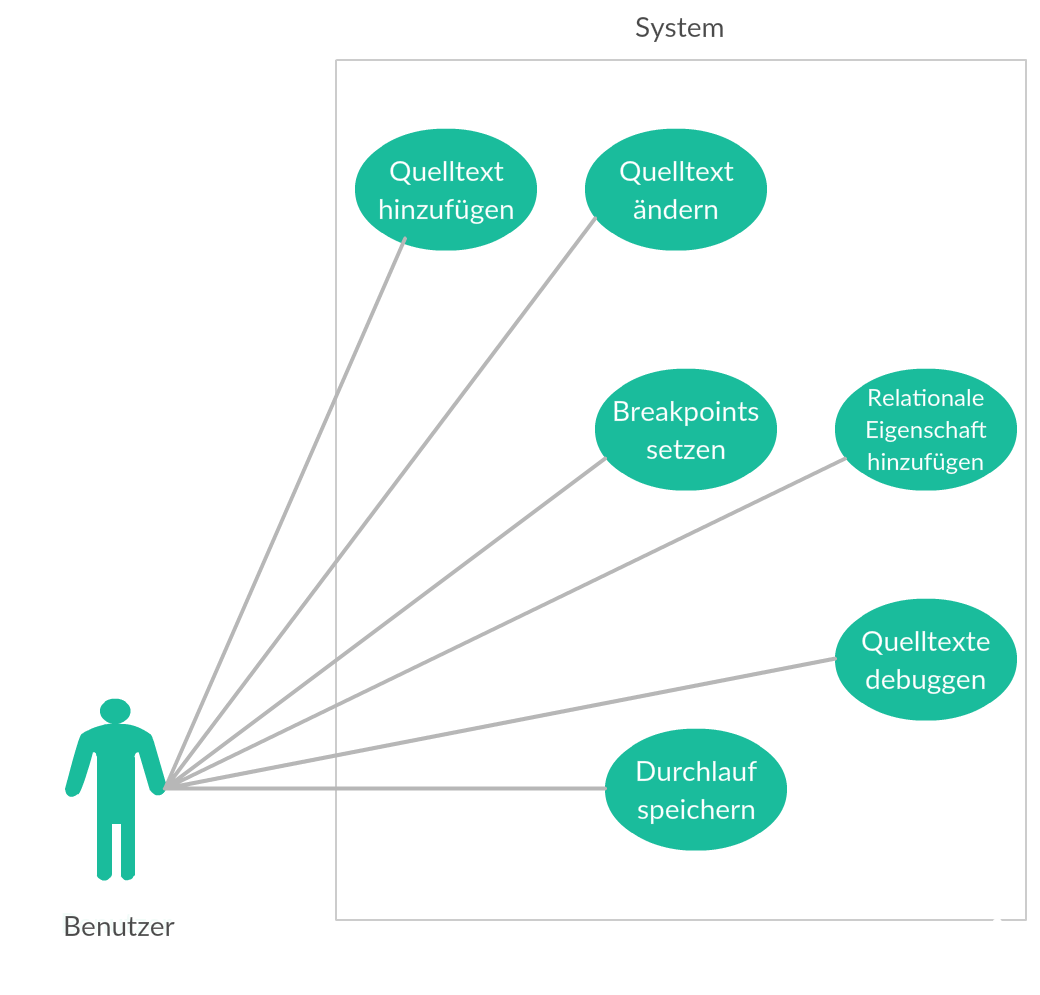
\includegraphics[width=0.7\textwidth]{Anwendungsfalldiagramm}
  \caption{Anwendungsfalldiagramm}
  \label{fig:Bild1}
\end{figure}

In allen Anwendungsfällen ist der Benutzer der einzige Akteur

\begin{itemize}
    \item [/AF10/] Hinzufügen von Programmen:\\ 
	Der Benutzer möchte einen Programmcode hinzufügen, auf welchen er über die Dateiverwaltung
	seines Betriebssystems zugreifen kann.\\
	Dazu wählt er die Schaltfläche \enquote{Datei} der Menüleiste. In der Menüansicht wählt er anschließend die Fläche \enquote{Programm hinzufügen}.\\
	Daraufhin öffnet sich die Dateiverwaltung seines Betriebssystems und der Benutzer fordert über diese den gewünschten Programmtext an.
	Das Programm erscheint in einem Eingabefenster.\\
	Hierbei ist folgende Ausnahme zu beachten: Besitzt das hinzuzufügende Programm mehr als 100 Zeilen, so benachrichtigt das Produkt den Benutzer über /A10/. Das Programm wird in jedem Fall hinzugefügt.\\
    
    \item [/AF20/] Ändern von Programmen:\\
    Der Benutzer möchte das von ihm hinzugefügte Programm ändern. Befindet er sich im \gls{Debugmodus}, muss er diesen zuvor abbrechen. \\
    Um den Code zu ändern, kann der Benutzer das Programm direkt im Fenster durch hineinklicken bearbeiten. Außerdem kann der Benutzer auch weitere Programme hinzufügen oder Programme entfernen.
    
    \item [/AF30/] Setzen von Breakpoints:\\
    Der Benutzer möchte einen \gls{Breakpoint} hinzufügen. Hierbei hat er die Möglichkeit, einen Breakpoint durch Doppelklick direkt in Zeilen im Programmtext zu setzen.\\
    Die zweite Möglichkeit ist das Setzen eines bedingten Breakpoints. Hierzu wählt der Benutzer die passende \enquote{+} Schaltfläche aus, fügt einen semantisch korrekten Ausdruck ein und wählt gegebenenfalls die zugehörigen Bereiche in den Programmen aus.
    
    \item [/AF40/] Hinzufügen von Watch-Expressions:\\
    Der Benutzer möchte eine \gls{Watch-Expression} bezüglich der von ihm hinzugefügten Programme hinzufügen. Dazu wählt er in der Benutzeroberfläche die Schaltfläche \enquote{+} unter Watch-Expressions aus. Hier gibt er einen semantisch korrekten %\gls{Watch-Expression} (siehe Kapitel 12) 
Ausdruck ein. Anschließend kann im selben Feld ein Bereich in einem oder mehreren der Programme angegeben werden, in dem das Produkt die Korrektheit der Watch-Expression untersucht. Wird einer oder mehrere dieser Bereiche leer gelassen, wird die Korrektheit der Watch-Expression während des gesamten Durchlaufs überprüft.
    
    \item [/AF50/] Codes debuggen: \\
                        %relationale Eigenschaften groß? (Rela...)
        Der Benutzer möchte zwei (oder mehr) Programmteile auf \glspl{Relationale Eigenschaft} (z.B. Nicht-Interferenz oder Äquivalenz) untersuchen. Dazu fügt er die zu untersuchenden Programme in das Produkt ein, setzt Breakpoints an relevanten Stellen und prüft seine Annahmen, wo die Programme sich unterscheiden könnten, mit Hilfe von Watch-Expressions oder \glsplgen{bedingter Breakpoint}. Gegebenenfalls verändert er den Programmtext seiner Programme noch einmal. Dann startet er den \gls{Debugger}. Dieser läuft automatisch bis zum jeweils nächsten (bedingten) Breakpoint durch. \\Der Benutzer hat dann die Möglichkeit, pro Zeile(n) oder pro Breakpoint vorzugehen. Die Ergebnisse der Variablen und der Auswertung der Watch-Expressions werden ihm dauerhaft angezeigt und nach jedem Weitergehen aktualisiert. Am Ende des Debug-Vorgangs werden ihm die Ausgabewerte aller Programme angezeigt.
    
    \item [/AF60/] Speichern eines Durchlaufs: \\
    Der Benutzer möchte einen von ihm durchgeführten Debug-Lauf speichern, um ihn später zu wiederholen, an dieser Stelle fortzusetzen oder an einen anderen Benutzer weiterzugeben. Dazu wählt er zu einem beliebigen Zeitpunkt, nachdem er mindestens einen zu debuggenden Programmtext hinzugefügt hat, im Dateimenü den Punkt \enquote{\gls{Konfigurationsdatei} speichern} aus. Anschließend kann der Benutzer den Speicherort der Konfigurationsdatei über ein Pop-Up Fenster auswählen.\\

\end{itemize}
\section{Globale Testfälle}

\subsection{Basisfunktionen}

\begin{itemize}
	\item[/T010/] Öffnen des Produkts
	\begin{itemize}
		\item Erfolgsvorbedingung: Das Produkt ist noch nicht geöffnet.
		\item Aktion: Das Produkt wird über das Terminal oder per Mausklick über das Produkt--Symbol aufgerufen.
		\item Reaktion: Das Produkt öffnet sich. Zu sehen sind die Menü-Leisten. Es sind nach dem Öffnen noch keine Programme des Nutzers eingebunden.
%		\item Verletzung der Vorbedingung: Das Programm lässt sich nur einmal öffnen. Folglich erscheint nur das bereits geöffnete Fenster wieder im Vordergrund.
	\end{itemize}
	
	\item[/T020/] Öffnen einer Textdatei
	\begin{itemize}
		\item Erfolgsvorbedingung: Das Produkt befindet sich im \gls{Editiermodus} und die auszuwählende Textdatei hat eine unterstützte Länge (vgl. /A10/).
		\item Aktion: Im Menü \enquote{Datei} wird der Menüpunkt \enquote{Textdatei öffnen} aufgerufen und die entsprechende Textdatei ausgewählt.
		\item Reaktion: Die ausgewählte Text-Datei wird in einem neuen Programm-Fenster \frage{??} eingefügt.
	\end{itemize}	

	\item[/T030/] Schließen des Produkts
	\begin{itemize}
		\item Erfolgsvorbedingung: Die Arbeit des Nutzers ist bereits gespeichert.
		\item Aktion: Es wird der Schließen-Button  oder der Menüpunkt \enquote{Beenden} im Menü \enquote{Datei} per Mausklick aufgerufen.
		\item Reaktion: Das Produkt beendet und schließt sich.
		\end{itemize}	
	
	\item[/T040/] Öffnen einer Konfiguration
		\begin{itemize}
		\item Erfolgsvorbedingung: Es ist aktuell keine Konfiguration geöffnet. Die auszuwählende Konfiguration ist korrekt abgespeichert und von unterstütztem Umfang (vgl. /A10/ und /A20/).
		\item Aktion: Im Menü \enquote{Datei} wird der Menüpunkt \enquote{Konfiguration öffnen} per Mausklick aufgerufen und die entsprechende \gls{Konfigurationsdatei} ausgewählt.
		\item Reaktion: Die Konfiguration wird angezeigt und der Nutzer kann die Arbeit daran fortsetzen.		
		\end{itemize}	
	
	\item[/T050/] Speichern einer Konfiguration
		\begin{itemize}
		\item Erfolgsvorbedingung: Die Konfiguration hat einen unterstützten Umfang (vgl. /A10/ und /A20/).
		\item Aktion: Im Menü \enquote{Datei} wird der Menüpunkt \enquote{Konfiguration speichern} per Mausklick aufgerufen.
		\item Reaktion:	Die aktuelle Konfiguration wird in einer Konfigurationsdatei abgespeichert.
		\end{itemize}	
	
	\end{itemize}

\subsection{Grundsätzliche Debug-Funktionen}

\begin{itemize}

	\item[/T060/] Setzen eines \glspl{Breakpoint} synchron in allen Textfenstern
	\begin{itemize}
		\item Erfolgsvorbedingung: Es sind mehrere Textfenster vorhanden. Die Stelle, an der der Breakpoint gesetzt werden sollen, ist in allen Textfenstern noch nicht von einem Breakpoint belegt und in allen Fenstern einem Befehl zugeordnet. 
		\item Aktion: Der linke Rand neben einem der Textfenster wird doppelt angeklickt.	
		\item Reaktion:	In allen vorhandenen Textfenstern wird auf derselben Höhe ein Breakpoint gesetzt.
	\end{itemize}		
	
	\item[/T070/] Löschen eines Breakpoints in einem Textfenster
		\begin{itemize}
		\item Erfolgsvorbedingung: Es ist an der entsprechenden Stelle ein Breakpoint gesetzt.	
		\item Aktion: Der zu entfernende Breakpoint wird einmal einfach angeklickt.
		\item Reaktion:	Der \gls{Breakpoint} wird erfolgreich entfernt, d.h. er ist weder zu sehen, noch hält das Programm zukünftig an der Stelle.
		\end{itemize}		
		
		
	\item[/T100/] Löschen aller Breakpoints eines Fensters
		\begin{itemize}
		\item Erfolgsvorbedingung: Es sind im entsprechenden Fenster mehrere Breakpoints vorhanden.
		\item Aktion: Es wird per Rechtsklick auf einen der Breakpoints des entsprechenden Fensters geklickt und die Option \enquote{Alle Breakpoints löschen} angeklickt.
		\item Reaktion:	Alle Breakpoints des Fensters werden gelöscht.
		\end{itemize}		
	
	\item[/T110/] Starten des \gls{Debugmodus}
		\begin{itemize}
		\item Erfolgsvorbedingung: Das Produkt befindet sich im \gls{Editiermodus}. Die zu untersuchenden Programme sind syntaktisch korrekt, d.h. es ergeben sich keine Fehler beim Kompilieren. Des Weiteren sind alle notwendigen Variableneingaben vorhanden und entsprechen dem Typ der jeweiligen Variable.
		\item Aktion: Der Play-Button wird angeklickt.
		\item Reaktion:	Das Produkt wechselt in den Debugmodus und läuft in allen Programmen bis zum jeweils ersten Breakpoint durch bzw. bis die Bedingung des ersten bedingten Breakpoints erfüllt wird.
		\end{itemize}		
	
	\item[/T120/] Abbrechen des Debugmodus
		\begin{itemize}
		\item Erfolgsvorbedingung: Das Produkt befindet sich im Debugmodus.
		\item Aktion: Der Stop-Button wird angeklickt.
		\item Reaktion: Das Produkt wechselt in den Editiermodus.		
		\end{itemize}		
	
	\item[/T130/] Halten des Debuggers an Breakpoints
		\begin{itemize}
		\item Erfolgsvorbedingung: Das Produkt befindet sich im Debugmodus. Es existiert ein Breakpoint in einem Textfenster.
		\item Aktion: Es gibt verschiedene Nutzer-Handlungen, durch die ein Breakpoint erreicht werden kann: Der Nutzer startet den Debugmodus mit Klick auf den Play-Button. Der Nutzer macht einen Schritt mittels Klick auf den Step-Button. Der Nutzer setzt das bisherige Debuggen fort mittels Klick auf den Continue-Button.
		\item Reaktion:	Das Produkt hält im entsprechenden Fenster in der Zeile des \glspl{Breakpoint} und zeigt die aktuellen Variablenwerte an. Die aktuell erfüllten Watch-Expressions werden farblich hinterlegt.
		\end{itemize}		
	
	\item[/T135/] Halten des Debuggers an \glsplgen{bedingter Breakpoint}
		\begin{itemize}
		\item Erfolgsvorbedingung: Das Produkt befindet sich im \gls{Debugmodus}. Es existiert ein bedingter Breakpoint mit syntaktisch korrekter und erfüllbarer Bedingung. 
		\item Aktion: Es gibt verschiedene Nutzer-Handlungen, durch die ein bedingter Breakpoint erreicht werden kann. Der Nutzer startet den Debugmodus mit Klick auf den Play-Button. / Der Nutzer macht einen Schritt mittels Klick auf den Step-Button. / Der Nutzer setzt das bisherige Debuggen fort mittels Klick auf den Continue-Button.
		\item Reaktion:	Der Debugger hält alle Programme an, sobald der bedingte Breakpoint in einem oder mehreren der Programme seine Bedingung erfüllt. Die aktuellen Variablenwerte werden angezeigt und aktuell erfüllte Watch-Expressions farblich hinterlegt.
		\end{itemize}	
	
	\item[/T140/] Verändern der Schrittgröße
		\begin{itemize}
		\item Erfolgsvorbedingung: Es ist ein Textfenster vorhanden.
		\item Aktion: Die Schrittgröße wird durch den Nutzer geändert, indem er in die entsprechende Box des Textfensters klickt. Dabei gibt er nur ganze Zahlen größer gleich Null und kleiner gleich der Länge des Programmtextes ein. \frage{??}
		\item Reaktion: Die Schrittgröße wird verändert angezeigt. Folgende Schritte haben die entsprechende Länge.
		\end{itemize}	
	
	\item[/T150/] Gleichzeitig in allen Textfenstern einen \gls{Schritt} der jeweils gewählten \gls{Schrittgroesse} machen
		\begin{itemize}
		\item Erfolgsvorbedingung: Das Produkt befindet sich im Debugmodus. Die zu testenden Textfenster (mindestens zwei) haben jeweils eine gültige Schrittlänge, und der Debugger ist in mindestens einem von ihnen noch nicht am Ende des Programmtextes angekommen.
		\item Aktion: Der Schritt-Button wird angeklickt.
		\item Reaktion:	In allen Fenstern wird ein Schritt der jeweiligen Größe ausgeführt. Die aktuellen Variablenwerte werden angezeigt und aktuell erfüllte Watch-Expressions farblich hinterlegt. Sind alle Programme an ihrem Ende angekommen, wechselt das Produkt zurück in den Editiermodus, zeigt aber weiterhin die letzten Werte der Variablen an.	
		\end{itemize}
	\item[/T160/] Einen \gls{Einzelschritt} in einem einzelnen Fenster machen
		\begin{itemize}
		\item Erfolgsvorbedingung: Das Produkt befindet sich im Debugmodus. Das zu testende Textfenster hat eine gültige Schrittlänge, und der Debugger ist noch nicht am Ende des Programmtextes angekommen.
		\item Aktion: Der Einzelschritt-Button des Textfensters wird angeklickt.
		\item Reaktion:	In dem Fenster wird ein Einzelschritt gemacht. Andere möglicherweise vorhandene Fenster verändern sich nicht. Die aktuellen Variablenwerte werden angezeigt und aktuell erfüllte Watch-Expressions farblich hinterlegt.
		\end{itemize}	
	
	\item[/T170/] Mittels \gls{Step-Over} eine Funktion nicht inspizieren
		\begin{itemize}
		\item Erfolgsvorbedingung: Das Produkt befindet sich im Debugmodus. Der nächste Befehl ist eine Funktion.
		\item Aktion: Der Step-Over-Button wird geklickt.
		\item Reaktion:	Das Produkt behandelt die Funktion wie einen einzelnen Befehl. Alle Befehle in der Funktion werden zwar ausgeführt, jedoch nicht als einzelne Befehle angezeigt.
		\end{itemize}	
	
	\item[/T180/] Mittels \gls{Step-Out} aus einer Funktion zurückkehren
		\begin{itemize}
		\item Erfolgsvorbedingung: Das Produkt befindet sich im Debugmodus. Der nächste auszuführende Befehl ist Teil einer Funktion.
		\item Aktion: Der Step-Out-Button wird angeklickt.
		\item Reaktion:	Das Produkt verlässt die aktuelle Funktion. Der Debugmodus wird anschließend außerhalb der Funktion fortgeführt. 	
		\end{itemize}	
	
	\item[/T190/] Korrektes Ausgeben der Ausgabewerte
		\begin{itemize}
		\item Erfolgsvorbedingung: In den Programmen sind Ausgabewerte definiert. Der Debugmodus wurde korrekt beendet und der Debugging-Prozess wurde erfolgreich durchgeführt.
		\item Aktion: Der Debugging-Prozess wird durch den roten Stopp-Knopf bzw. durch das Ausführen des letzten Schrittes in beiden Programmen beendet.
		\item Reaktion:	In den Ausgabewerte-Fenstern werden die Ausgabewerte der jeweiligen Programme angezeigt.	
		\end{itemize}	
	
	\item[/T200/] Korrektes Auswerten der \glspl{Watch-Expression}
		\begin{itemize}
		\item Erfolgsvorbedingung: Die angegebenen Watch-Expressions sind nach Definition valide. 
		\item Aktion: Das Produkt wird durch klicken des grünen Startsymbols in den Debugmodus versetzt. 
		\item Reaktion:	Die Watch-Expressions werden als wahr oder falsch ausgewertet und entsprechend markiert.	
		\end{itemize}	
	
	\item[/T210/] Korrektes Anzeigen der Zwischenwerte von Variablen
		\begin{itemize}
		\item Erfolgsvorbedingung: Der Programmcode ist nach Definition der Sprache Wlang valide. Die Variablen kommen im Programmcode vor.
		\item Aktion: Das Produkt wird durch klicken des grünen Startsymbols in den Debugmodus versetzt.
		\item Reaktion:	Die aktuellen Werte der Variablen werden im Variableninspektor angezeigt.Nach jedem auswerteten Befehl werden diese Werte aktualisiert.	
		\end{itemize}	
	
	
\end{itemize}

\subsection{Watch-Expressions}

\begin{itemize}

	\item[/T220/] Hinzufügen einer \gls{Watch-Expression}
		\begin{itemize}
		\item Erfolgsvorbedingung: Der Benutzer hat bereits mindestens ein zu debuggendes Programm hinzugefügt.
		\item Aktion: Der Nutzer wählt im Block \enquote{Watch-Expressions} das \enquote{+}-Symbol aus. Anschließend gibt er in das Feld eine semantisch korrekte Watch-Expression ein.
		\item Reaktion:	Die Watch-Expression wird hinzugefügt und deren Auswertung beginnt im Debugmodus direkt, im Editiermodus hingegen sobald der Debugmodus gestartet wird.
		\end{itemize}	
\newpage
	\item[/T230/] Löschen einer Watch-Expression
		\begin{itemize}
		\item Erfolgsvorbedingung: Eine Watch Expression existiert.
		\item Aktion: Der Nutzer wählt bei der zu löschenden Watch-Expression das Menüfeld aus. Anschließend wählt er den Eintrag \enquote{Löschen}.
		\item Reaktion:	Die Watch-Expression wird direkt gelöscht und nicht mehr ausgewertet.
		\end{itemize}	
	
	\item[/T240/] Bearbeiten einer Watch-Expression
		\begin{itemize}
		\item Erfolgsvorbedingung: Eine Watch-Expression existiert.
		\item Aktion:              Der Nutzer wählt per Mausklick das Eingabefeld der zu bearbeitenden Watch-Expression.
                                           Anschließend ändert er die Watch-Expression ab, sodass eine syntaktisch und 
                                           semantisch korrekte Watch-Expression im Feld sichtbar wird. Der Benutzer bestätigt 
                                           seine Eingabe.
		\item Reaktion:	           Die Watch-Expression wird hinzugefügt und deren Auswertung beginnt im Debugmodus 
                                           direkt, im Editiermodus hingegen sobald der Debugmodus gestartet wird.	
		\end{itemize}	
                                            
	
	\item[/T250/] Hinzufügen einer Bereichsbindung
		\begin{itemize}
		\item Erfolgsvorbedingung: Eine Watch-Expression existiert.
		\item Aktion: Der Nutzer wählt über das Optionenfeld der Watch-Expression die Option \enquote{an Bereich binden} aus. Dann gibt er im erscheinenden Menü die erste und letzte Zeile des Bereichs in jedem der zu debuggenden Programme an, an den die Watch-Expression gebunden wird. 
		\item Reaktion:	Die Watch-Expression wird während des Debuggens nur noch ausgewertet, wenn sich eines der Programme im jeweiligen Bereich befindet. Beim Anzeigen der Bereichsbindung(/T270/) wird diese angezeigt. 
		\end{itemize}	
\newpage
	\item[/T260/] Löschen einer Bereichsbindung
		\begin{itemize}
		\item Erfolgsvorbedingung: Eine Watch-Expression existiert und wurde bereits an einen Bereich gebunden. 
		\item Aktion: Der Nutzer wählt über das Optionenfeld der Watch-Expression die Option \enquote{von Bereich lösen} aus.
		\item Reaktion:	Die Bereichsbindung wird aufgehoben und die Watch-Expression wird während des Debuggens dauerhaft überprüft und ausgewertet.
		\end{itemize}	
	
	\item[/T270/] Anzeigen einer Bereichsbindung
		\begin{itemize}
		\item Erfolgsvorbedingung: Eine Watch-Expression existiert und wurde bereits an einen Bereich gebunden. 
		\item Aktion: Der Nutzer bewegt die Maus über die Watch-Expression oder wählt über das Optionenfeld der Watch-Expression die Option \enquote{an Bereich binden} aus. 
		\item Reaktion:	Das Produkt zeigt die existierende Bereichsbindung an.  
		\end{itemize}	
	
		
\end{itemize}
\subsection{Bedingte Breakpoints}

\begin{itemize}

	\item[/T280/] Hinzufügen eines \glsplgen{bedingter Breakpoint}
		\begin{itemize}
		\item Erfolgsvorbedingung: Der Benutzer hat bereits mindestens ein zu debuggendes Programm hinzugefügt.
		\item Aktion: Der Nutzer wählt im Block \enquote{Bedingte Breakpoints} das \enquote{+}-Symbol aus. Anschließend gibt er in das Feld eine semantisch korrekten bedingten Breakpoint ein.
		\item Reaktion:	Der bedingte Breakpoint wird hinzugefügt und dessen Auswertung beginnt im Debugmodus direkt, im Editiermodus hingegen sobald der Debugmodus gestartet wird.	
		\end{itemize}	
\newpage	
	\item[/T290/] Löschen eines bedingten Breakpoints
		\begin{itemize}
		\item Erfolgsvorbedingung: Ein bedingter Breakpoint existiert.
		\item Aktion: Der Nutzer wählt bei den zu löschenden bedingten Breakpoint das Menüfeld aus. Anschließend wählt er den Eintrag \enquote{Löschen}.
		\item Reaktion:	Der bedingte Breakpoint wird direkt gelöscht und nicht mehr ausgewertet.	
		\end{itemize}	
	
	\item[/T300/] Bearbeiten eines bedingten Breakpoints
		\begin{itemize}
		\item Erfolgsvorbedingung: Ein bedingter Breakpoint existiert.
		\item Aktion:              Der Nutzer wählt per Mausklick das Eingabefeld des zu bearbeitenden bedingten Breakpoints.
                                           Anschließend ändert er den bedingten Breakpoint so ab, sodass ein syntaktisch und 
                                           semantisch korrekter Breakpoint im Feld sichtbar wird. Der Benutzer bestätigt 
                                           seine Eingabe.
        	\item Reaktion:            Der bedingte Breakpoint wird hinzugefügt und dessen Auswertung beginnt im Debugmodus direkt, 
                                           im Editiermodus hingegen sobald der Debugmodus gestartet wird.			
		\end{itemize}	
	
	\item[/T310/] Hinzufügen einer Bereichsbindung
		\begin{itemize}
		\item Erfolgsvorbedingung: Ein bedingter Breakpoint existiert.
		\item Aktion: Der Nutzer wählt über das Optionenfeld des bedingten Breakpoints die Option \enquote{an Bereich binden} aus. Dann gibt er im erscheinenden Menü die erste und letzte Zeile des Bereichs in jedem der zu debuggenden Programme an, an den der bedingte Breakpoint gebunden wird. 
		\item Reaktion:	Der bedingte Breakpoint wird während des Debuggens nur noch ausgewertet, wenn sich eines der Programme im jeweiligen Bereich befindet. Beim Anzeigen der Bereichsbindung(/T270/) wird diese angezeigt. 
		\end{itemize}		
\newpage	
	\item[/T260/] Löschen einer Bereichsbindung
		\begin{itemize}
		\item Erfolgsvorbedingung: Ein bedingter Breakpoint existiert und wurde bereits an einen Bereich gebunden. 
		\item Aktion: Der Nutzer wählt über das Optionenfeld des bedingten Breakpoints die Option \enquote{von Bereich lösen} aus.
		\item Reaktion:	Die Bereichsbindung wird aufgehoben und der bedingte Breakpoint wird während des Debuggens dauerhaft überprüft und ausgewertet.
		\end{itemize}	
	
	\item[/T330/] Anzeigen einer Bereichsbindung
		\begin{itemize}
		\item Erfolgsvorbedingung: Ein bedingter Breakpoint existiert und wurde bereits an einen Bereich gebunden. 
		\item Aktion: Der Nutzer bewegt die Maus über den bedingten Breakpoint oder wählt über das Optionenfeld des bedingten Breakpoints die Option \enquote{an Bereich binden} aus. 
		\item Reaktion:	Das Produkt zeigt die existierende Bereichsbindung an.  
		\end{itemize}	
	
		
\end{itemize}

\subsection{Variableneingabe}



\begin{itemize}

\item[/T340/] Angeben des Startwerts einer Variablen
		\begin{itemize}
		\item Erfolgsvorbedingung: Das Produkt befindet sich im Editiermodus. Es ist ein Programmtext angegeben, der einen Startwert für mindestens eine Variable erfordert.
		\item Aktion: Es wird in das Feld \enquote{Eingabewerte} geklickt und die Variablenzuweisung eingegeben.
		\item Reaktion: Die Eingabewerte werden so angezeigt, wie der Nutzer sie eingegeben hat.
		\end{itemize}	
\newpage	
\item[/T350/] Angeben einer Wertespanne für den zufälligen Startwert einer Variablen
		\begin{itemize}
		\item Erfolgsvorbedingung: Das Produkt befindet sich im Editiermodus. Es ist ein Programmtext angegeben, der einen Startwert für mindestens eine Variable erfordert.
		\item Aktion: Über das Menü \enquote{Einstellungen} wird der Menüpunkt \enquote{Variablenwerte} aufgerufen. Dort wird die Variable hinzugefügt und ihre Wertespanne dem Datentyp entsprechend eingegeben.
		\item Reaktion: Die Wertespanne wird gespeichert und beim Starten des Debugmodus wird ein zufälliger Wert innerhalb der Wertespanne als Startwert genutzt.
		\end{itemize}
	
\end{itemize}

\subsection{Menü-Funktionen}

Ein Item bezeichnet hier jeweils eine Einheit innerhalb eines Submenüs, zum Beispiel eine Watch-Expression innerhalb des Watch-Expression-Blocks oder ein Paar aus einer Variable und ihrem aktuellen Wert in der Variablenausgabe.

\begin{itemize}

	\item[/T360/] Verändern der Item-Reihenfolge
		\begin{itemize}
		\item Erfolgsvorbedingung: Im \gls{Variableninspektor} befinden sich mindestens zwei Variablen.
		\item Aktion: Durch \enquote{Drag and Drop} verändert der Benutzer die Reihenfolge der Variablen.
		\item Reaktion:	Die verschobene Variable wird je nach Aktion weiter oben beziehungsweise unten im Variableninspektor angezeigt.
		\end{itemize}	
	
	\item[/T370/] Ein- und Ausblenden von Variablen
		\begin{itemize}
		\item Erfolgsvorbedingung: Die Programmtexte ist nach Definition der Sprache Wlang valide. Die ein-/auszublendenden
                                           Variablen kommen in den Programmen vor.
                                           %  Präziser ausdrücken? "[...] Variablen wurden deklariert"
                \item Aktion:              Über das Menü \enquote{Einstellungen} wird der Menüpunkt \enquote{Variablen ein-/ausblenden} 
                                           aufgerufen. Dort wird ausgewählt, welche im Programm vorkommenden Variablen ein- oder
                                           ausgeblendet werden sollen.
		\item Reaktion:		   Die Zwischenwerte der einzublendenden Variablen werden korrekt angezeigt.
                                           Die Zwischenwerte der auszublendenden Variablen werden nicht angezeigt.
		\end{itemize}	
	
	\item[/T380/] Korrektes Anzeigen des Scrollbalkens
		\begin{itemize}
		\item Erfolgsvorbedingung: Es befinden sich mindestens so viele Variablen im \gls{Variableninspektor}, dass das dafür vorgesehene Feld in der Benutzeroberfläche ausreicht.
		\item Aktion: Keine Aktion des Benutzers notwendig.
		\item Reaktion:	Rechts im Feld des \glspl{Variableninspektor} 	wird ein Scrollbalken angezeigt, welchen der Benutzer verschieben kann um alle Variablen einzusehen.
		\end{itemize}	
	
\end{itemize}


\newpage
\section{Systemmodelle}
%Architektur, Verhalten, usw
\begin{figure}[h] 
  \centering
     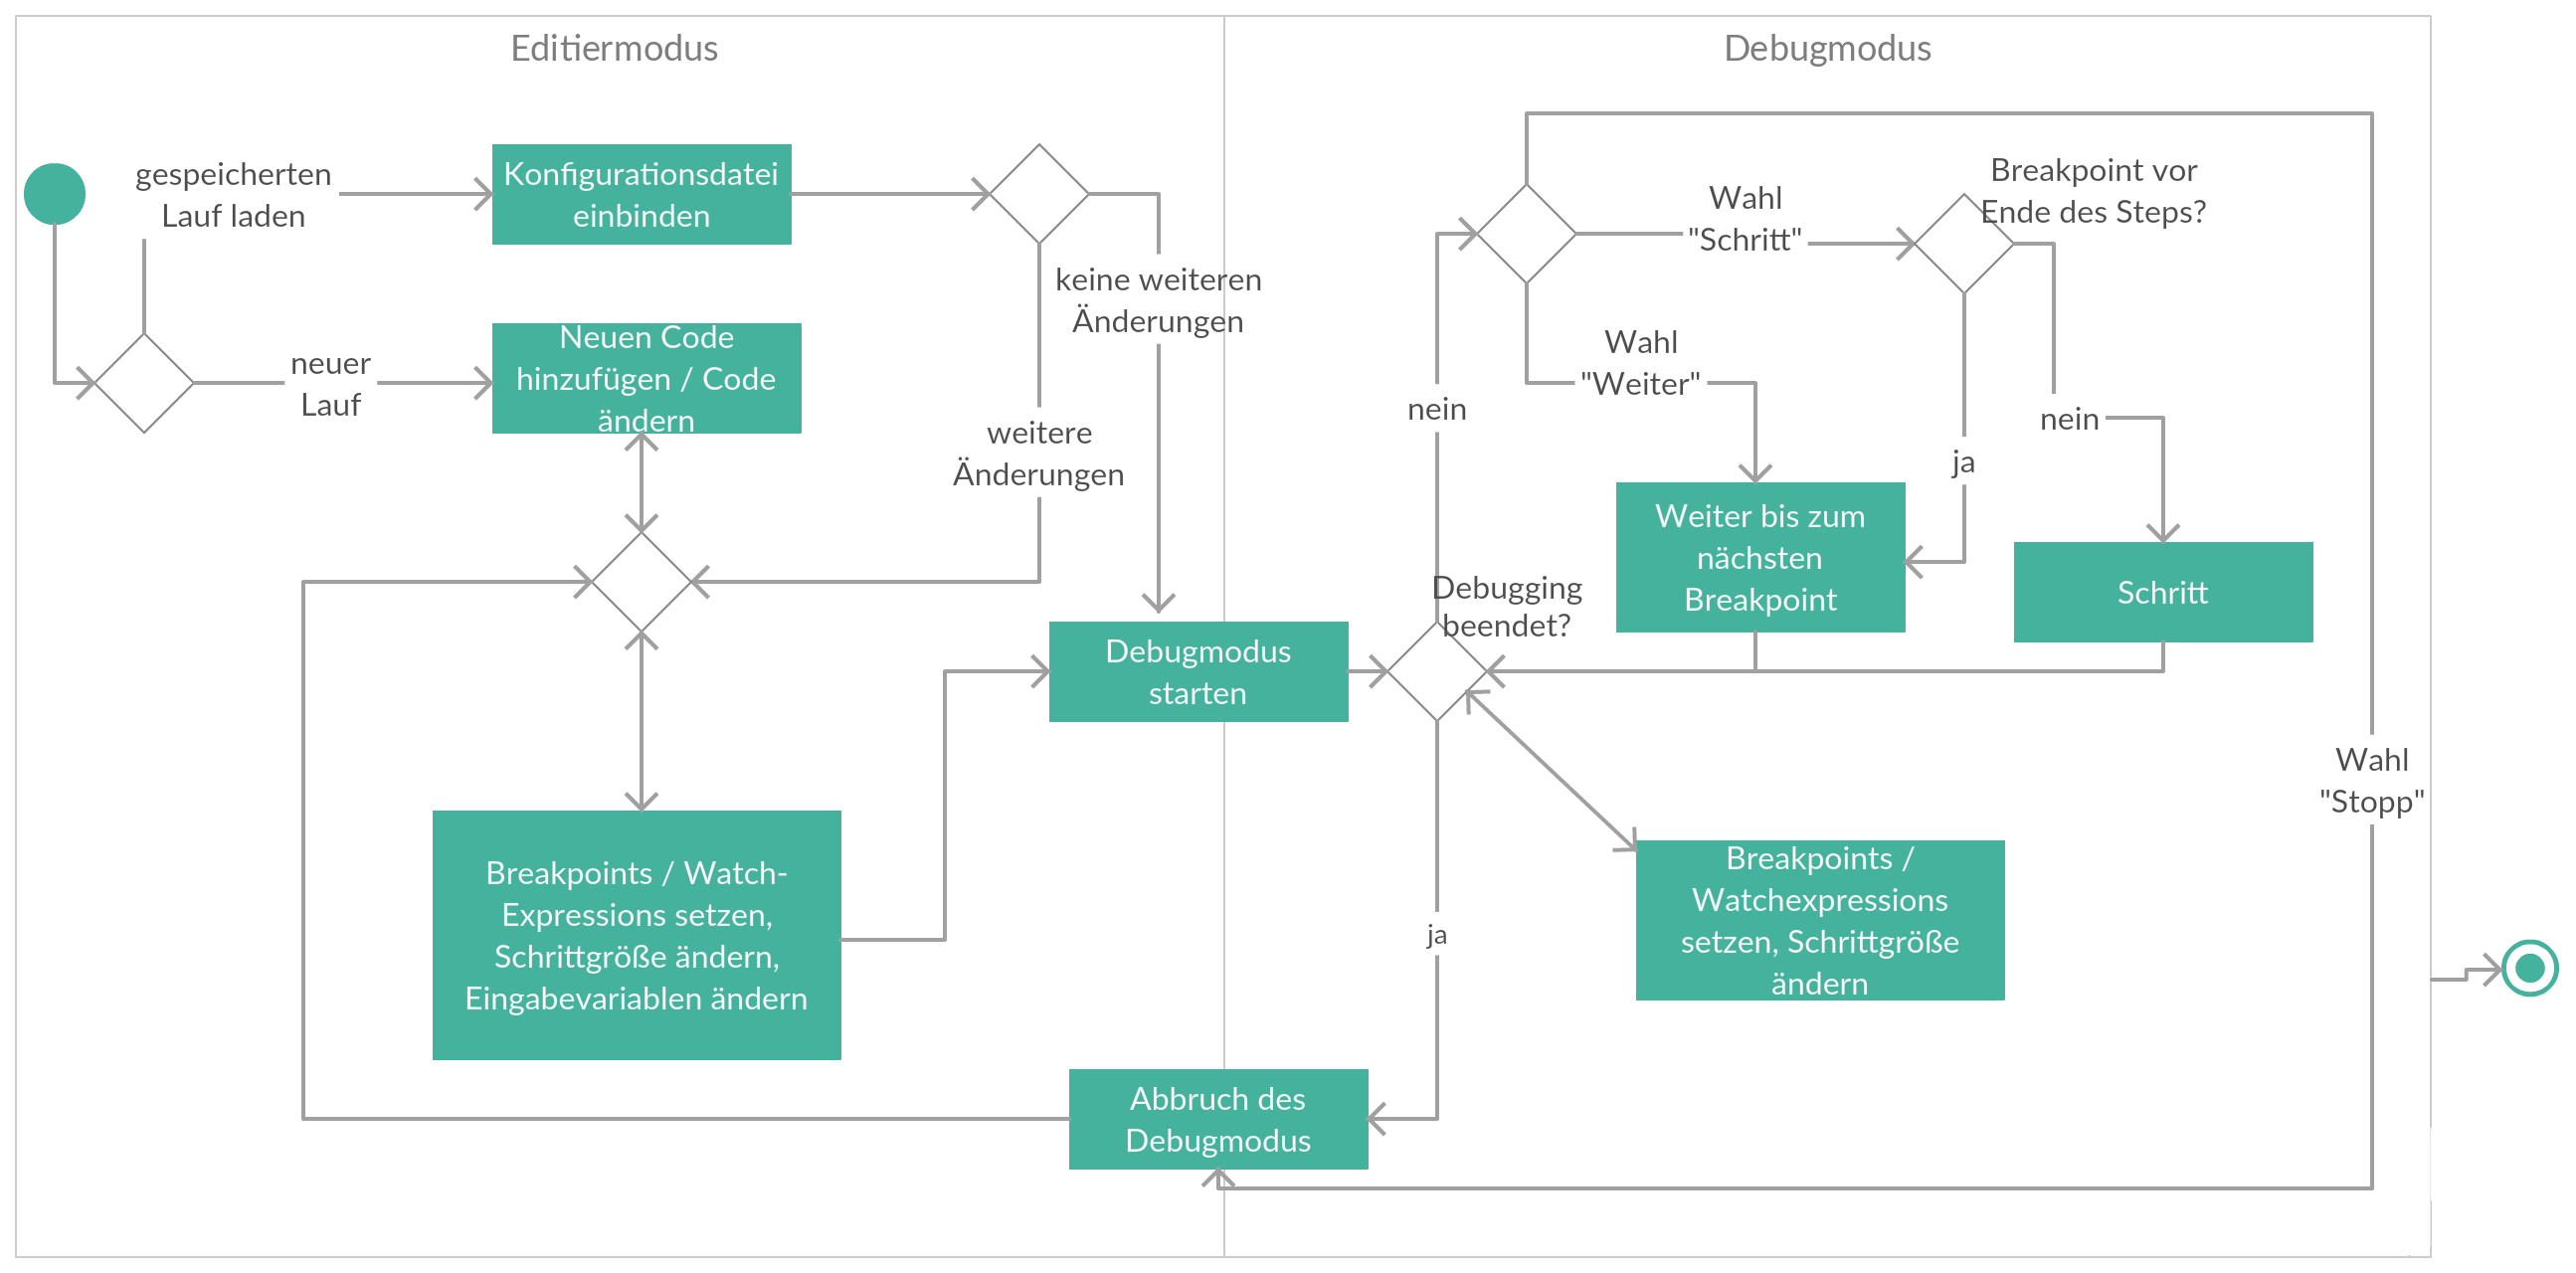
\includegraphics[width=1.0\textwidth]{Aktivitaetsdiagramm}
  \caption{Aktivitätsdiagramm}
  \label{fig:Bild2}
\end{figure}
\vspace{0.7cm}
Das Aktivitätsdiagramm stellt die möglichen Reihenfolgen der Interaktion des Benutzers mit dem Produkt dar. \\
Bindet der Benutzer direkt nach Start des Programms eine \gls{Konfigurationsdatei} eines früheren Laufs ein, kann er diesen Lauf direkt starten oder vorher Änderungen an den Eingaben und Programmen vornehmen. \\
Die Aufteilung in \gls{Editiermodus} und \gls{Debugmodus} zeigt, dass das Ändern und Hinzufügen von Programmen und Ändern der Eingabevariablen nicht während des Debugmodus möglich sind. Das Ändern von (bedingten) \glspl{Breakpoint}, \glspl{Watch-Expression} und der Schrittgröße ist auch im Debugmodus möglich, allerdings nur zwischen den ausgeführten Schritten und an Breakpoints. \\
Nach manuellem Abbruch oder nach kompletter Durchführung eines Debug-Laufs kehrt das Produkt zum Editiermodus zurück. Die vorherigen Eingaben bleiben bestehen, sodass die Wiederholung des Laufs ohne Änderungen direkt möglich ist. Ebenso kann der Benutzer wieder Änderungen an den Eingabevariablen und den Programmen vornehmen.\\
Das Beenden des Produkts ist an jeder Stelle möglich.

\newpage

\begin{figure}[!ht]
	\centering
	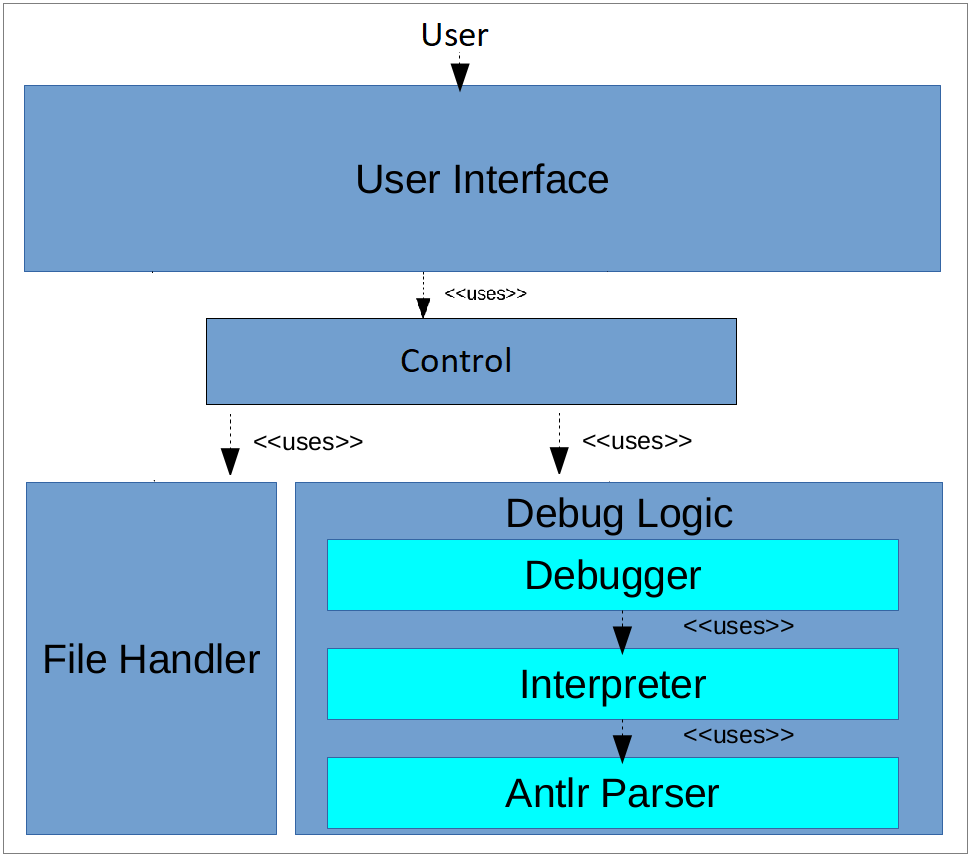
\includegraphics[width=1.0\textwidth]{Architektur}
	\caption{Systemarchitektur}
	\label{fig:Bild3} 

\end{figure}
\vspace{0.7cm}
	\paragraph{User Interface} Das User Interface ist der Teil des Produktes, den der Benutzer sieht und mit dem er direkt interagieren kann. Somit dient dieser Teil dem Nutzer als Schnittstelle für Kontrolle und Ansicht. 
	\paragraph{File Handler} Der File Handler stellt Funktionalität zum Laden, Einlesen und Speichern von Dateien bereit. Diese Dateien speichern Sprache, die Konfiguration eines Laufes oder Einstellungen des Nutzers. Neben dem eigentlichen Einlesen übernimmt der File Handler auch die Aufgabe, die Dateien entprechend zu parsen und zu interpretieren. Diese Funktionalität wird vom User Interface genutzt, falls der Nutzer die entsprechende Anweisung gibt. Für eine Änderung des Speicherformates müsste also nur der File Handler durch einen anderen ersetzt werden.
	\paragraph{Debug Logic} Die Debug Logic stellt die eigentlichen Debugmechanismen und die Interpretation der zu debugenden Programme sowie die Logik der \glspl{Watch-Expression} und \glsplgen{bedingter Breakpoint} zur Verfügung. Sie ist unterteilt in: 
	\subparagraph{Debugger} Der Debugger nutzt die vom \gls{Interpreter} erzeugten Informationen, um Watch-Expression und bedingte Breakpoints auszuwerten, sowie die üblichen Debugmechanismen zu steuern.
	\subparagraph{Interpreter} Der Interpreter nutzt den Syntax-Baum, den der Antlr Parser erzeugt, um damit den Programmablauf der zu debuggenden Programme auszuführen. 
	\subparagraph{Antlr Parser} Der Antlr Parser enthält die von Antlr generierten Elemente zur Erzeugung des Syntaxbaums aus den eingegebenen Quelltexten.
	
	
\newpage
\section{Benutzeroberfläche}
%Gui-Skizzen, Erklärungen der Menüs, usw
\begin{figure}[!ht] 
    \vspace{-10pt}
    \centering
       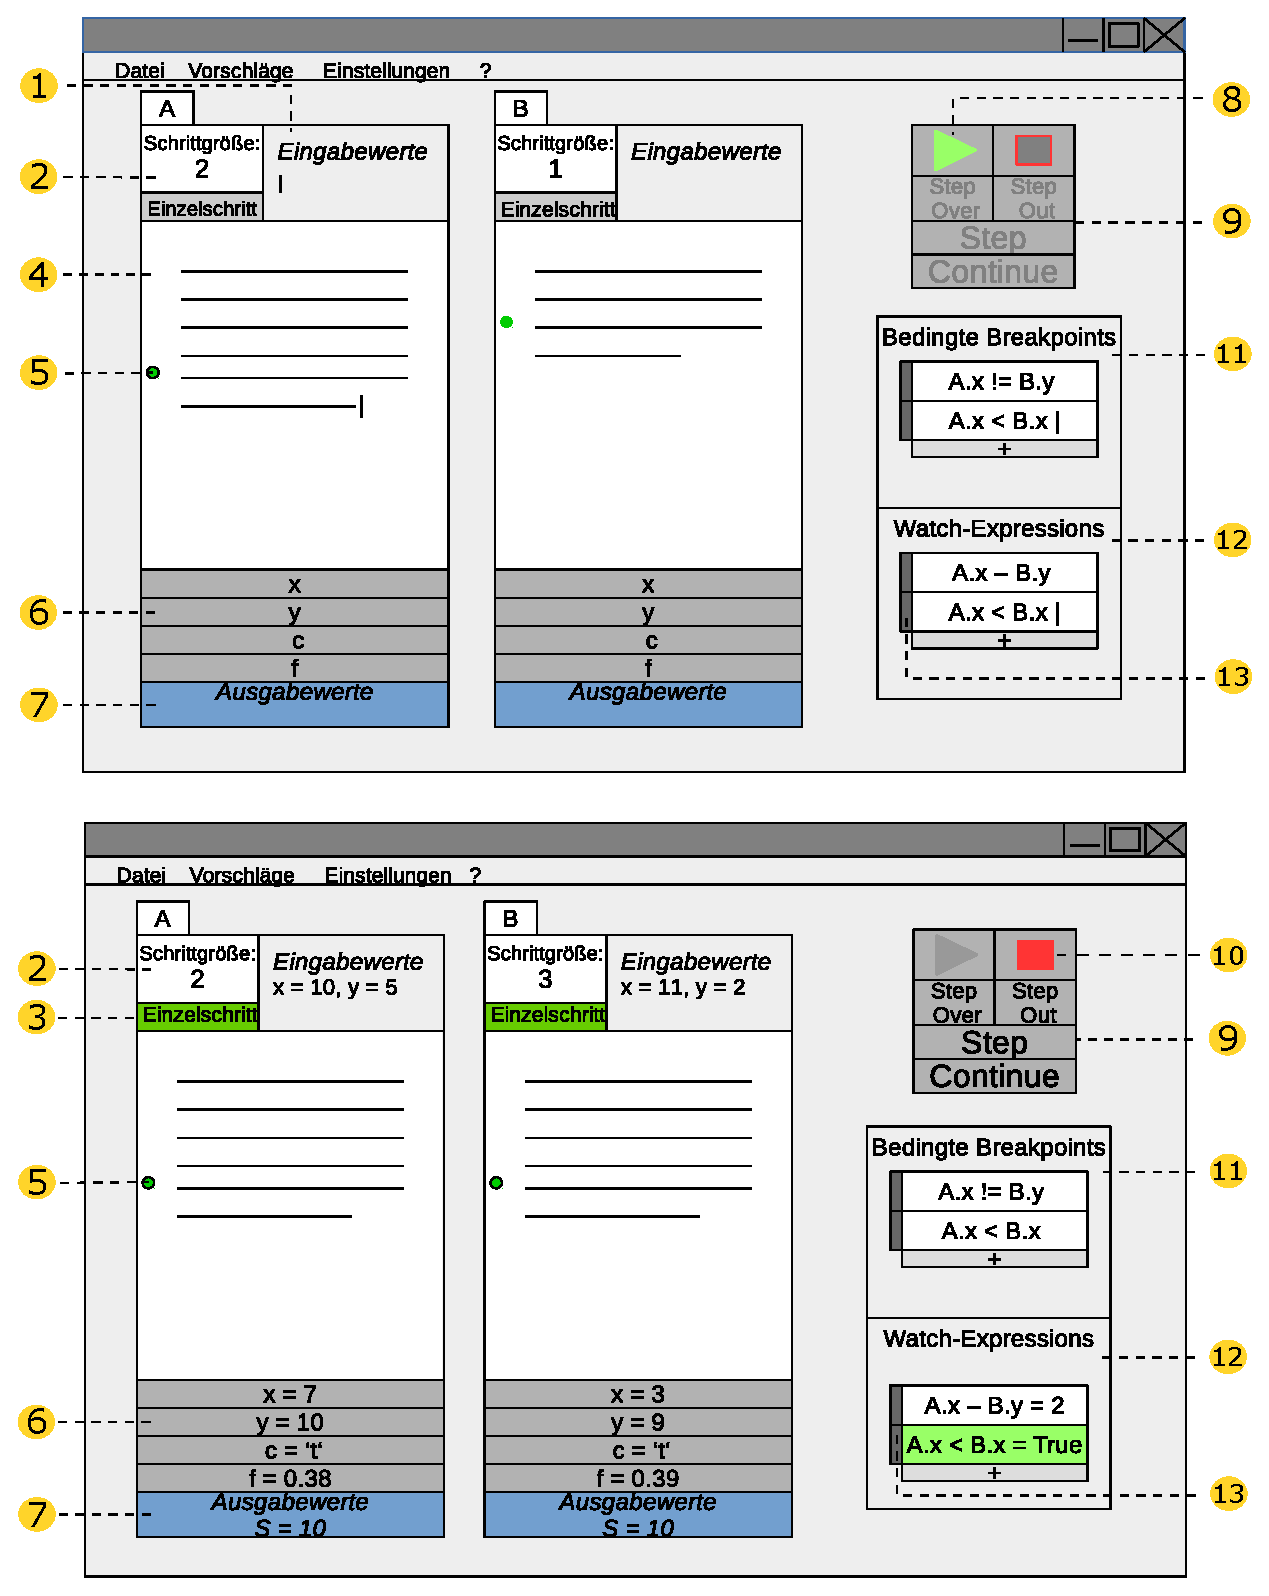
\includegraphics[width=0.95\textwidth]{skizzeFull_v2.eps}
       \caption{
         Benutzeroberfläche des Produktes im Editiermodus (oben) und im Debugmodus
         (unten)
       }
    \label{fig:Bild4}
\end{figure}

\newpage
    \subsection{Beschreibung der Oberfläche}
        Befindet sich das Produkt im \gls{Editiermodus}, so können die Programme über die 
        Eingabefenster (4) bearbeitet werden.
        Durch Verändern der Texte im Bereich \enquote{Eingabewerte} (1) können Werte der Eingabevariablen
        spezifiziert, gelöscht und verändert werden. 
        Die Schaltflächen \enquote{Step} und \enquote{Continue}, sowie \enquote{\gls{Einzelschritt}} können in diesem Modus nicht betätigt
        werden (Bereich 9). Betätigung der Startschaltfläche (8) verursacht den Übergang des Produkts in den \gls{Debugmodus}.
        
        Befindet sich das Produkt im Debugmodus, können die Programme nicht mehr
        bearbeitet werden.
        Die Schaltflächen \enquote{Step}, \enquote{Continue} und \enquote{Einzelschritt}, sowie \enquote{Step Over} und \enquote{Step Out} können
        benutzt werden, um die Programme zu debuggen (Bereich 9). Dabei führt \enquote{Step} einen \gls{Schritt} aus (entsprechend der \gls{Schrittgroesse}) und \enquote{Continue} führt die Programme bis zum jeweils nächsten Breakpoint aus. \glspl{Breakpoint} (5) können am Rand der Eingabefenstern (4) per Mausklick gesetzt werden.
        Betätigung der Stoppschaltfläche (10) verursacht den Übergang in den Editiermodus.

        In beiden Modi können \glspl{bedingter Breakpoint} (11) und \glspl{Watch-Expression} (12) durch Betätigung der jeweiligen 
        \enquote{+}-Schaltflächen hinzugefügt werden. Über die Optionsschaltflächen (13) auf der linken Seite der Watch-Expression und bedingter Breakpoint können Wirksamkeitsbereiche der Watch-Expressions und Breakpoints
        spezifiziert werden.\\
     \subsection{Beschreibung der Menüs}
     Die Benutzeroberfläche bietet die folgenden Menüs:
     \begin{itemize}
     \item[Datei] Dieses Menü enthält die Menüeinträge \enquote{Neu}, \enquote{Konfigurationsdatei laden}, \enquote{Konfigrationsdatei speichern} und \enquote{Neues Programm hinzufügen}. Außerdem kann das Produkt über dieses Menü beendet werden.
     \item[Vorschläge] In diesem Menü befinden sich die Menüeinträge, um Vorschläge für Watch-Expressions, bedingte Breakpoints und Eingabevariablen anzufordern.
     \item[Einstellungen] Über dieses Menü können Grundeinstellungen des Produkts, wie die Sprache der Benutzeroberfläche, angepasst werden.
     \item[Hilfe] Das Hilfemenü \enquote{?} stellt Hinweise zur Benutzung des Produkts zur Verfügung.
     \end{itemize}
       
\section{Anforderungen an die Entwicklungsumgebung}
Bei der Erstellung des Aktivitäts- und Anwendungsfalldiagramms wurde die Freie Version des Online-Diagramm-Editors \href{https://creately.com/}{Creately} verwendet.
Für die Entwicklung in Java werden die Java-Entwicklungsumgebungen IntelliJ\textsuperscript{\textcopyright} (2017.2.6) und Eclipse\textsuperscript{\textcopyright} Oxygen verwendet.

        
\section{Zeit- und Ressourcenplanung}
% Tabelle mit Phasendaten (Ideen sammeln, Einzelarbeit, Ideen zusammentragen, Überarbeitung, Abgabe Vorversion, Kolloquium/Abgabe Finalversion)
\subsection{Zeitliche Gesamtplanung}
Der Umfang des Moduls beträgt 9 ECTS, das entspricht 270 Arbeitsstunden pro Teilnehmer. Diese teilen sich wie folgt auf die Phasen der Softwareentwicklung auf: \\
\begin{itemize}
\item Definitionssphase\\ \textit{06.11.2017 - 26.11.2017}: 27h/Teilnehmer 
\item Entwurfsphase\\ \textit{27.11.2017 - 24.12.2017}: 81h/Teilnehmer
\item Implementierungsphase\\ \textit{08.01.2018 - 04.02.2018}:  81h/Teilnehmer
\item Qualitätssicherungsphase\\ \textit{19.02.2018 - 11.03.2018}: 54h/Teilnehmer
\item Abnahme und Präsentation\\ \textit{12.03.2018 - 25.03-2018}:  27h/Teilnehmer
\end{itemize}

\subsection{Phasenverantwortliche:}
Definitionsphase: Chiara Staudenmaier\\
Entwurfsphase: Joana Plewnia, Benedikt Wagner\\
Implementierungsphase: Pascal Zwick\\
Qualitätssicherungsphase: Etienne Brunner\\
Präsentation/Abnahme: Ulla Scheler\\
\subsection{Vorraussichtliche zeitliche Feinplanung}
\subsubsection{Definitionsphase}
\textit{bis 08.11.} Sammeln der Inhalte\\
\textit{bis 15.11.} Formulierung der Punkte im Pflichtenheft in Einzelarbeit\\
\textit{bis 17.11.} Gemeinsame Überarbeitung\\
\textit{17.11. 11:30 Uhr} Abgabe der vor-finalen Version des Pflichtenhefts\\
\textit{bis 24.11.} Gemeinsame Überarbeitung\\
\textit{24.11. 11:30 Uhr} Abgabe der finalen Version des Pflichtenhefts \\

\subsubsection{Entwurfsphase}
\textit{bis 03.12.} Fertigstellung der Einteilung des Systems in Pakete und Unterpakete und Festlegung der Schnittstellen derer \\
\textit{bis 10.12.} Fertigstellung der Einteilung der Pakete in Klassen und definieren der Methoden und Attribute derer \\
\textit{bis 17.12.} Fertigstellung der Paket- und Klassenbeschreibungen und des vorläufigen Entwurfsdokumentes\\
\textit{22.12.} Abgabe des endgültigen Entwurfs

\subsubsection{Implementierungsphase}
\textit{bis 14.01.} Fertigstellung der Dateiverwalter und des \glspl{Interpreter}. Beginn an Front- und Backend\\
\textit{bis 21.01.} Fertige, aber noch nicht funktionelle Benutzeroberfläche. Bereitstellung einiger Methoden des Backends für diese\\
\textit{bis 28.01.} Vollständige Implementierung des Backends und ein funktionierendes Frontend\\
\textit{bis 04.02.} Ende und Abgabe der Implementierung des Programms

\subsubsection{Qualitätssicherungsphase}
\textit{bis 28.02.} Komponententest\\
\textit{bis 07.03.} Integrationstest\\
\textit{bis 11.03.} Systemtest, gegebenenfalls Abnahmetest\\

\subsubsection{Abnahme und Präsentation }
\textit{bis 16.03.} Einarbeiten der Anmerkungen aus dem letzten Kolloquium \\
\textit{bis NN} Anfertigung der Abschlusspräsentation
\newpage
\section{Ergänzungen}
%Sprache
\subsection{Sprache}
Die Programmiersprache, in der die zu debuggenden Programme verfasst sind, wird im Folgenden als \enquote{WLang} (WHILE-Language) bezeichnet. 
\paragraph{Klassifikation der Sprache} WLang ist prozedural und imperativ, nicht objektorientiert und nicht einrückungsbasiert.
\paragraph{Elemente der Sprache}
WLang unterstützt die folgenden primitiven Datentypen:
\begin{itemize}
\item  32-bit Ganzzahlen: \texttt{int}
  \item  64-bit Ganzzahlen: \texttt{long}
 \item  32-bit IEEE 754 Fließkommazahlen: \texttt{float}
 \item   64-bit IEEE 754 Fließkommazahlen: \texttt{double}
  \item  Einzelnes Zeichen: \texttt{char}
  \item  Wahrheitswert: \texttt{boolean}
\end{itemize}
Zudem sind bis zu dreidimensionale Arrays dieser Datentypen möglich.
Ferner unterstützt WLang die folgenden Kontrollstrukturen:
\begin{itemize}
\item Funktionen und Prozeduren, also Unterprogramme mit oder ohne Rückgabewert.
\item Bedingte Ausführung: \texttt{if, else if, else}
\item Schleifen: \texttt{while}
\end{itemize}
Es muss in jedem Programm eine \texttt{main}-Routine vorhanden sein, von der die Ausführung ausgeht. Routinen, die aufgerufen werden, müssen darüber stehen. Kommentare können sowohl zeilenweise (\texttt{//}) als auch zeilenübergreifend (\texttt{/*Kommentar*/}) benutzt werden. Sämtliche Variablen müssen innerhalb einer Routine stehen. Auch Rekursion ist möglich.
\newpage

\paragraph{Syntax der Sprache}
Die Syntax von WLang ist angeleht an gängige Programmiersprachen wie C oder Java. Im folgenden Listing ist ein Beispielprogramm aufgeführt. 

\begin{verbatim}
void doUselessStuff() { //Prozedur ohne Rückgabe
    int a = 0;
}
float divide(float x, float y) { //Funktion mit Rückgabewert
    if(y != 0)	
        return x / y;
    return -1; //Rückgabe
}
int main(int j, int k)
{
    int a; //Deklaration
    a = 1; //Zuweisung
    long x = 100000L; 
    int b = 2; // Deklaration mit Initialisierung
    int[j + k ] myInts; \\Arraydeklaration
    char[4] myChars = {'a','b','c','d'};
    if(j < k) {
        int i = 0;
        while(i < j) {
            myInts[i] = 0; //Arrayzugriff
            i = i + 1;
        }	
    } else if(j == k) {
        return 0;
    } else
        return -1;
    doUselessStuff(); //Routinenaufruf
    float z = divide(3.0f*k / 1.1f);
    return z + j;
}
\end{verbatim}
\newpage
\subsection{Syntax der Watch-Expressions und bedingten Breakpoints}
Die Syntax der \glspl{Watch-Expression} und \glsplgen{bedingter Breakpoint} ist durch folgende kontextfreie Ableitungsregeln gegeben: \\\\
<WatchExpression> $\rightarrow$ <BooleanExpression> | <Term>\\\\
<BedingterBreakpoint> $\rightarrow$ <BooleanExpression>\\\\<BooleanExpression> $\rightarrow$ <Term> < <Term> 
| <Term> > <Term> |\\ <Term> >= <Term>|<Term> <= <Term>| <Term> == <Term>| \\<Term> != <Term>\\\\
<Term> $\rightarrow$ <Term> / <Term> 
| <Term> * <Term> |\\ <Term> - <Term>|<Term> + <Term>| <Term> \% <Term> | (<Term>) |<Atom>\\\\

Wobei ein <Atom> ein fester Wert eines Datentyps (z.B. \texttt{5, 'c', true}) oder eine Variable der Form <Programmbezeichner>.<Variablenname> (z.B. \texttt{A.x} für Variable x in Programm A) ist. \% steht für die Modulo-Operation.\\
Das heißt Watch-Expressions werten sich zu einem beliebigen Wert aus, während sich bedingte Breakpoints immer zu einem Wahrheitswert auswerten.


\newpage
\printglossary[style=altlist, toctitle=Glossar]


\end{document}
\grid
